\begin{figure}[t]
\begin{subfigure}[h]{0.48\linewidth}
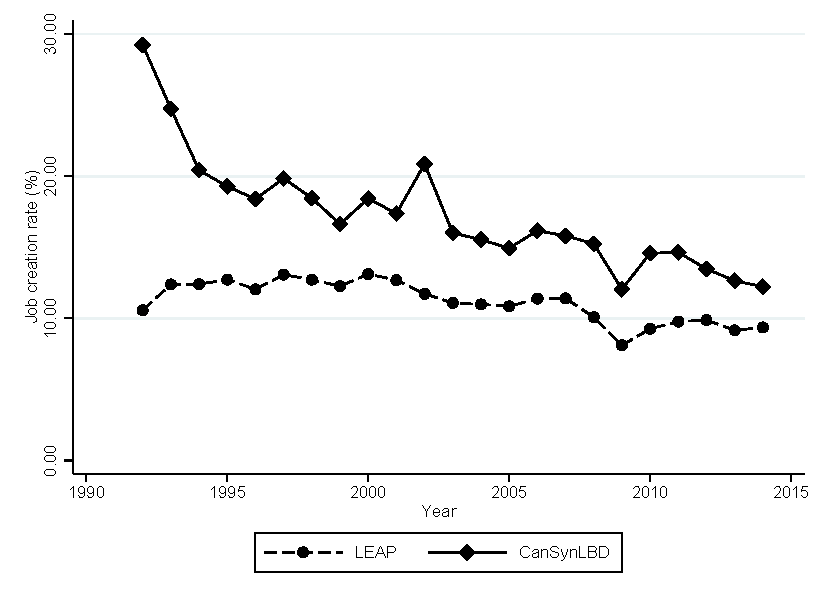
\includegraphics[trim=0 40 0 0,clip, width=\linewidth]{graphs/Job_creation_rate_by_year_private_bw.pdf}
%\caption{CanSynLBD}
\end{subfigure}
\hfill
\begin{subfigure}[h]{0.48\linewidth}
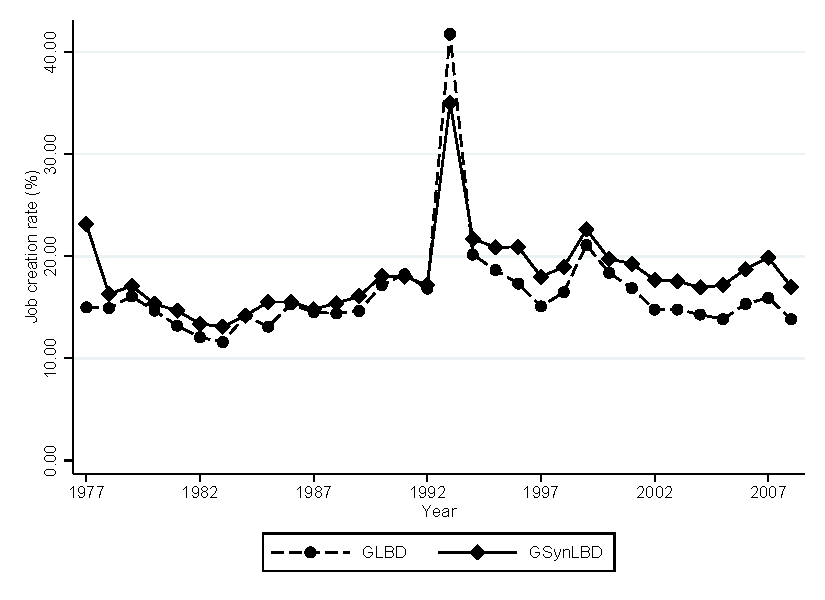
\includegraphics[trim=0 40 0 0,clip,width=\linewidth]{graphs/Job_creation_rate_by_year_bw_GsynLBD.pdf}
%\caption{GSynLBD}
\end{subfigure}\\
\begin{subfigure}[h]{0.48\linewidth}
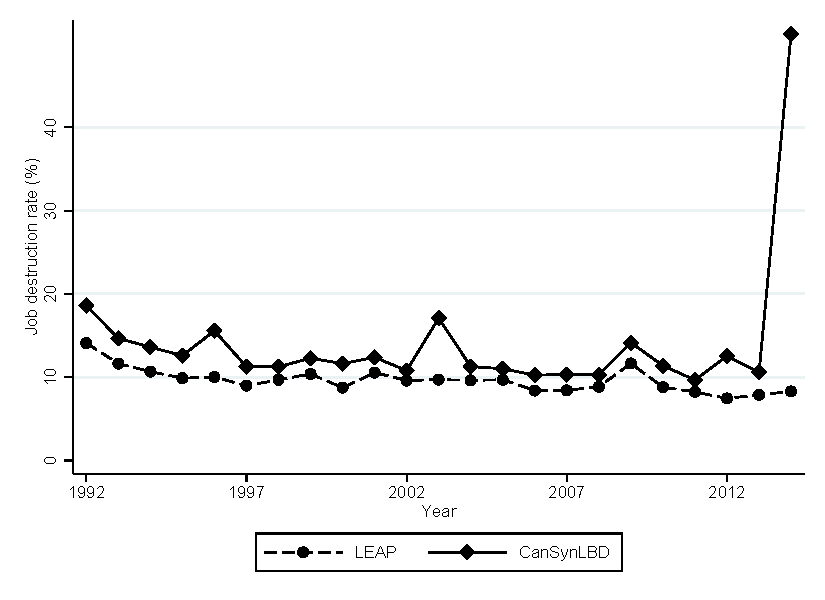
\includegraphics[trim=0 0 0 -20,clip,width=\linewidth]{graphs/Job_destruction_rate_by_year_private_bw.pdf}
\caption{CanSynLBD}
\end{subfigure}
\hfill
\begin{subfigure}[h]{0.48\linewidth}
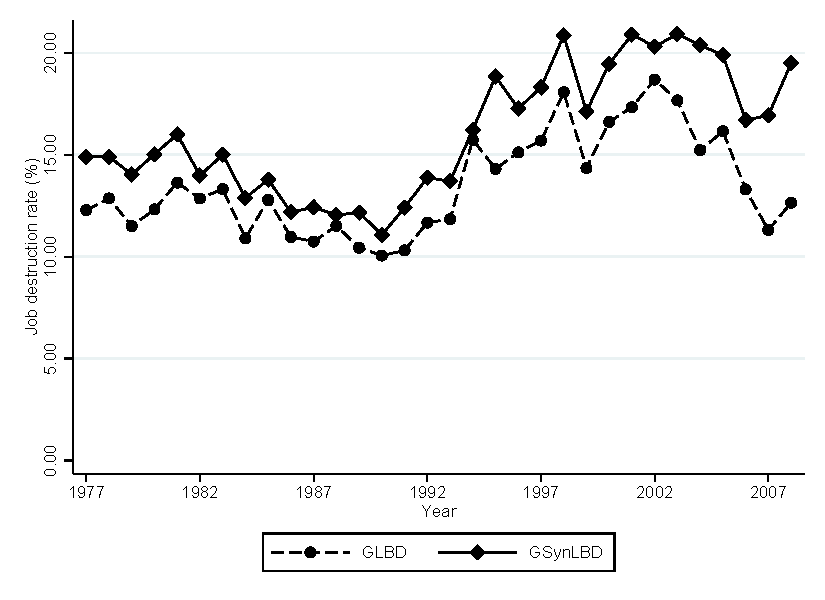
\includegraphics[trim=0 0 0 -20,clip,width=\linewidth]{graphs/Job_destruction_by_year_bw_GsynLBD.pdf}
\caption{GSynLBD}
\end{subfigure}%
\caption{Job creation rates (upper panels) and job destruction rates (lower panels) by year.}\label{fig:job_flows}
\end{figure}
